\chapter{Task 01: Ising Model}
\section{Task Description}
The Ising model, initially examined in d-dimensional regular lattices, has been demonstrated to undergo phase transitions in certain types of complex networks as well. This task aims to review various analytical results that have been established \cite{crit_fen_review} and to simulate the dynamics of the Ising model on networks.
\section{Mathematical Model}
The ferromagnetic Ising model on a network of $N$ nodes and adiacency matrix $A$ is described in its most general form by the Hamiltonian:
\begin{equation*}
    \mathcal{H}(\mathbf{s}) = - \sum_{i < j}\, J_{i,j}\,s_i\cdot s_j - \sum_{i}\, h_i\,s_i
\end{equation*}
where $\mathbf{s} = (s_1, \cdots s_N) \in \{\pm 1\}^N$ is the spin configuration of the nodes, the couplings $J_{i,\,j}$ describe the pairwise spin interactions and $h_i$ is a site-dependent external field.
In the following, it will be always assumed $J_{i,\,j} \equiv 1\cdot A_{i,\,j}$ (only nearest neighbours interactions, of homogeneous strength) and $h_i \equiv h$ (homogeneous external field), so that the Hamiltonian simplifies to:
\begin{equation}
        \mathcal{H}(\mathbf{s}) = - \sum_{i < j}\, A_{i,j}\,s_i\cdot s_j - h\cdot \sum_{i}\,s_i.
        \label{eq:ising_Hamiltonian}
\end{equation}
The network is surrounded by a heat bath at temperature $T = \frac{1}{\beta} $ ($k_B \equiv 1$). The partition function $Z$ and the free energy $F$ are given by:
\begin{equation*}
    Z\left(T, \{A_{i,\,j}\}, h, N\right) = \sum_{\mathbf{s}}\, e^{-\beta\, \mathcal{H}(\mathbf{s})} \quad F = -\frac{1}{\beta}\, \text{ln}[Z]
\end{equation*}
The most relevant thermodynamic quantities are the internal energy $E$, the magnetization $M$, the specific heat $C$ and the magnetic susceptibility $\chi$:

\begin{align*}
E &= \mathbbm{E}[\mathcal{H}(\mathbf{s})], &
C &= \left( \frac{\partial E}{\partial T} \right)_{h} \equiv \frac{\mathbbm{E}[E^2] - \mathbbm{E}[E]^2}{T^2} \\
M &= \mathbbm{E}\left[\sum_{i} s_i \right] \equiv \left( \frac{\partial F}{\partial h} \right)_{\beta}, &
\chi &= \left( \frac{\partial M}{\partial h} \right)_{T} = -\left( \frac{\partial^2 F}{\partial^2 h} \right)_{T} \equiv \frac{\mathbbm{E}[M^2] - \mathbbm{E}[M]^2}{T}
\end{align*}


\noindent A mean field approximation predicts that the existence of a disordered phase depends on the moments $\left\langle k^n\right\rangle$ of the network degree distribution. Specifically, a homogeneous mean field approximation yields the critical temperature
\begin{equation} \label{eq:hom_mean_field}
    T_C^{\text{hom. MF}} =\,\left\langle k \right \rangle.
\end{equation}
[Appendix \ref{app:mean_field}] contains the explicit calculation of this formula. According to mean field approximation, the critical temperature is expected to increase with the average degree, which indicates that adding more connections between the nodes helps in maintaining long-range order. The more precise heterogeneous (or degree-based) mean field approximation yields instead:
\begin{equation} \label{eq:het_mean_field}
    T_C^{\text{het. MF}} =\,\frac{\left\langle k^2 \right \rangle}{\left\langle k \right \rangle}.
\end{equation}
In particular, the latter formula is derived under the assumption that the network is uncorrelated, i.e. the nearest neighbour degree distribution is supposed to be that of the configuration model: $P_{n.n.} (k)=\frac{k\cdot P(k)}{<k>}$.
A refined estimation of the critical temperature on uncorrelated networks is found with the replica approach (see \cite{analytical_ising}): 
\begin{equation}
    T_C^{replica} = \left[ -\frac{1}{2}\,\text{ln}\left[2- \frac{\left\langle k \right\rangle}{\left\langle k^2 \right\rangle}\right]\right]^{-1}
\label{eq:replica}    
\end{equation}
The order parameter of the transition is the average magnetization per site, $s$:
$$
s := \frac{M}{N} = \mathbbm{E}\left[\frac{\sum_{i}\,s_i}{N}\right]
$$
which is zero in the disordered phase ($T>T_C$), non-zero in the ferromagnetic  phase $(T<T_C)$ and monotonically decreasing with temperature. Also, the energy $E(T)$ is expected to have an inflection point at $T=T_C$, and the response functions $C$ and $\chi$ are both supposed to peak at $T=T_C$.

\section{Numerical Simulations}
For simulations, I chose to focus on scale free networks $P(k) \sim k^{-\gamma}$, in particular the Barabasi - Albert (BA) network of parameters $N,\, m$ where N is the number of nodes and $m$ is the number of links attacched for each new node. This choice was motivated by the fact that article \cite{numeric_ising} could be used for comparison. The degree distribution for such a network is asymptotically given by $P(k) \sim k^{-3}$. Since one can only deal with finite size networks, finite size effects must be taken into account in the formulas $[\ref{eq:hom_mean_field}$, $\ref{eq:het_mean_field}, \ref{eq:replica}$].
The finite size of the network implies the existence of a cutoff degree $k_{max}(N)$, so the right estimation of the moment $\left\langle k^n \right \rangle$ is given by
\begin{equation*}
    <k^n> = \sum_{k=m}^{k_{max}(N)}\, k^n\,P(k),
\end{equation*}
where the cutoff $k_{max}(N)$ is defined such that the probability of having a node of degree $k>k$ in a network of size $N$ is less than one. With an elementary calculation one can verify that $k_{max}(N)= m\cdot N^{\frac{1}{\gamma -1}}$, which reduces to $k_{max} = m\cdot \sqrt{N}$ for a BA network.
The average degree is left unchanged by the finite size correction:  $\left \langle k \right \rangle = 2m$, whereas the second moment changes to $\left \langle k^2 \right \rangle \simeq m^2\,\text{ln}(N)$ \cite{analytical_ising}. Hence, the critical temperatures given by the mean field formulas are:
\begin{equation}
    T_C^{\text{hom. MF}} = 2m, \quad \quad T_C^{\text{het. MF}} \simeq \frac{m}{2}\,\text{ln}(N)
\end{equation}
As mentioned earlier, these formulas are derived for uncorrelated networks, which BA networks are not. Nevertheless, the authors of \cite{numeric_ising} verified through simulations that BA networks also align well with these formulas.
The heterogeneous mean field approximation predicts a logarithmic increase of the temperature with the network size, which means that in the thermodynamic limit ($N\rightarrow +\infty$) the network is expected to be ferromagnetic at all temperatures.
The homogeneous mean field is overly simplistic and fails to predict this behaviour. 
\bigskip \newline \noindent
The algorithm I implemented to simulate the Ising dynamic is the Metropolis-Hasting. As a preliminary check, I first used my code to simulate the Ising model on a regular $2d$ lattice of $N =400$ nodes [Appendix, figures: \ref{fig:2d_relaxation} and \ref{fig:2d_scaling}]. and then on BA networks of the same size.
Computational time for the simulations on BA was much higher: for comparison, obtaining the scaling of thermodynamic quantities with temperature [Appendix, figure: \ref{fig:2d_scaling}] took $12$ minutes, whereas obtaining the same data for BA [Figure: \ref{fig:ising_BA_scaling}] took on average $1h$). Handling the adiacency matrix of the network in sparse format brought a significant performance improvement, but still the computations were long. \medskip \newline \noindent
For estimating the critical temperature, I initially planned to derive an estimate from each of the four thermodynamic quantities ($E, \left\langle s \right\rangle, C, \chi$) and then average them. However, I found that the peak temperature of the specific heat $C$ was systematically lower than the peak temperature of the magnetic susceptibility $\chi$ [see Figure: \ref{fig:ising_BA_scaling}]. Among the two peaks, the latter was closer to the theoretical temperature value. This discrepancy was not observed in preliminary simulations on a $2d$ regular lattice, indicating that it is not an artifact of my code. In fact, this same behavior was also observed by my colleague D. Wellingut \cite{dw}. Therefore, I averaged the temperatures obtained from the magnetization and the magnetic susceptibility, disregarding the other two. The final results of my simulations are shown in [Figure: \ref{fig:final_ising}]. The critical temperature estimated from the simulations is systematically lower than the theoretical predictions, but at least the dependence on $m$ is similar.
\begin{figure}[H]
    \centering
    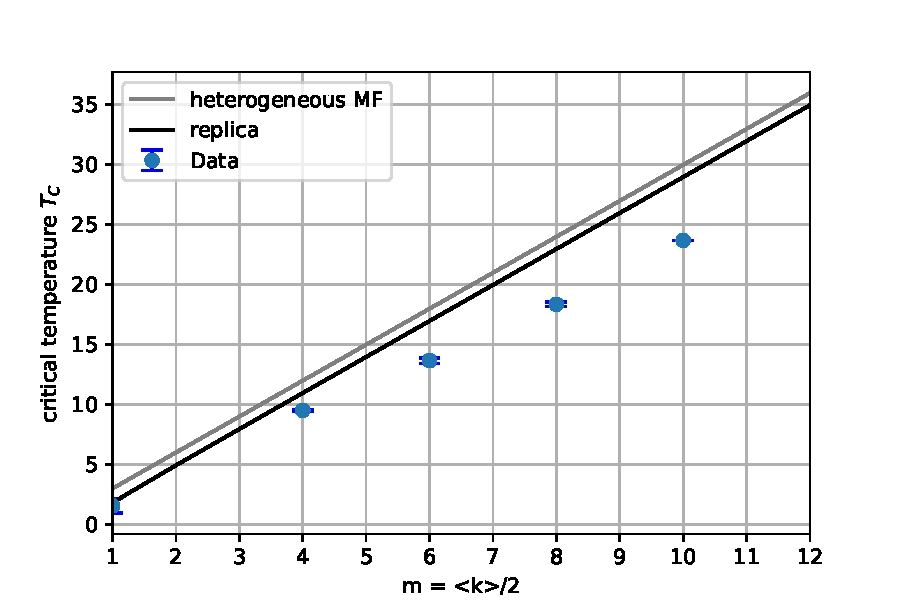
\includegraphics[width=0.7\linewidth]{latex_source/images/ising/BA_temperatures.pdf}
    \caption{Scaling of the critical temperature with the minimum degree, for BA networks of $400$ nodes. The data refers to the critical temperature estrapolated from the magnetization and the magnetic susceptibility peak.}
    \label{fig:final_ising}
\end{figure}

\begin{figure}[H]
    \centering
    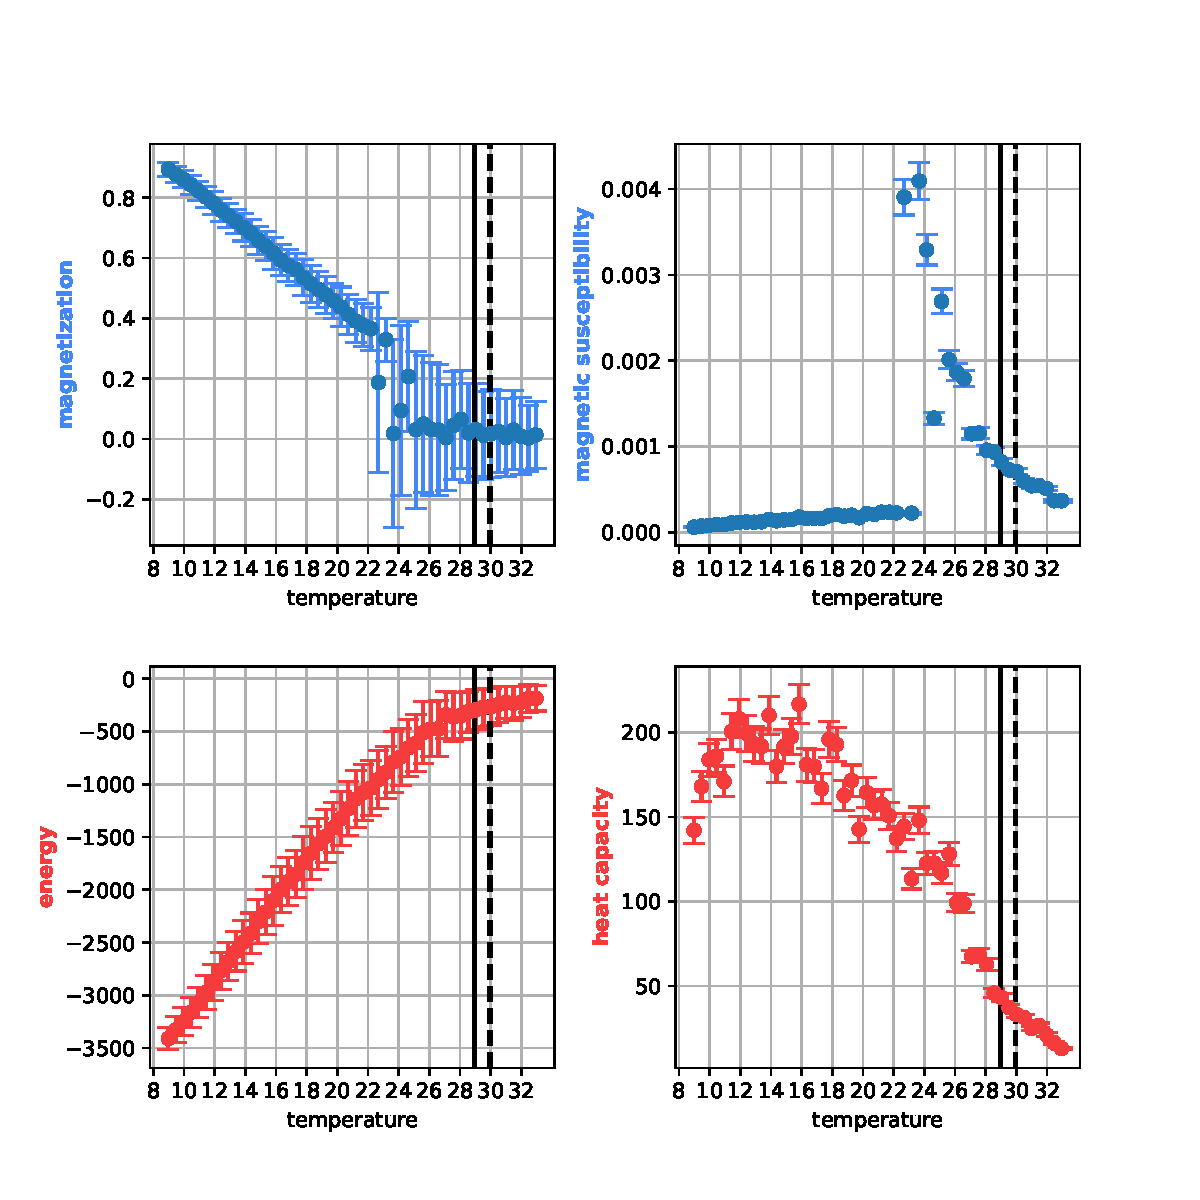
\includegraphics[width=\linewidth]{latex_source/images/ising/BA_scaling_num_nodes_400_t_points_50_steps_700_m_10_ti_8.99_tf_32.95.pdf}
    \caption{Scaling of thermodinamic quantities with temperature. BA network with $N=400$ and $m=10$. Metropolis algorithm has been run with $1500$ equilibration steps and $700$ sweep steps. The dashed line is the heterogeneous mean field temperature \ref{eq:het_mean_field}, while the solid line is the replica temperature \ref{eq:replica}. The peaks of the two response fuctions do not coincide.}
    \label{fig:ising_BA_scaling}
\end{figure}

\newpage
\section*{Appendix}
\addcontentsline{toc}{section}{Appendix}
\subsection*{Homogeneous mean-field calculation for $T_C$ } \label{app:mean_field}
{\small
The mean field approximation consists in neglecting the pairwise spin correlations $
    \text{corr}(s_i,\,s_j) = (s_i - \left\langle s_i \right \rangle)\cdot (s_j - \left\langle s_j \right \rangle)\simeq 0 $.
Moreover, the homogeneous mean field supposes that the average magnetization on each node is the same for all nodes $\left\langle s_i\right\rangle \equiv \left \langle s \right \rangle$. We start from the Ising Hamiltonian $H\{\mathbf{s}\} = -\frac{1}{2}\, \sum_{i,\,j}\,A_{i,\,j}\,s_i\cdot s_j - h\cdot\sum_{i}\,s_i$ and write the identity: 
\begin{align*}
    s_i\cdot s_j &= [s_i - \left\langle s \right \rangle + \left\langle s \right \rangle]\cdot [s_j - \left\langle s \right \rangle + \left\langle s \right \rangle] \\
    &= (s_i - \left\langle s \right \rangle)\cdot (s_j-\left\langle s \right \rangle) + (s_i + s_j) \left\langle s \right \rangle - \left\langle s \right \rangle^2 \simeq (s_i + s_j) \left\langle s \right \rangle - \left\langle s \right \rangle^2
\end{align*} where the latter is obtained disregarding the correlation term. With this substitution, the Hamiltonian becomes 
\begin{equation*}
    H \simeq\frac{1}{2}\,\left\langle s \right \rangle^2\,N\,\left\langle k \right \rangle - \sum_i\,s_i\cdot (\left\langle k \right \rangle\left\langle s \right \rangle + h)=: H^{MF}(\mathbf{s})
\end{equation*}
This expression can be now used to compute the partition function $Z$ and, consequently, the free energy per site $f= F/N$:
\begin{align*}
    Z^{MF} &= \sum_{\mathbf{s}}\, e^{-\beta H^{MF}(\mathbf{s})} = e^{-\beta \frac{N \left\langle k \right \rangle\left\langle s \right \rangle^2}{2}}\, \sum_{\mathbf{s}}\, e^{\beta\left[(<k><s> + h)\sum_l\,s_l\right]} \\
    &= e^{-\beta \frac{N <k><s>^2}{2}}\, \prod_{i=1}^{N}\, \left[ \sum_{s = \pm 1}\, e^{\beta(<k>+h)\,s_i} \right] \\
    &= e^{-\beta \frac{N \left\langle k \right \rangle\left\langle s \right \rangle^2}{2}}\,\left[2\,\text{cosh}\left[\beta(\left\langle s \right \rangle\left\langle k \right \rangle+h)\right]\right]^N \\
   f^{MF}&= \frac{F^{MF}}{N} = - \frac{1}{N\beta}\text{ln}Z^{MF} = \frac{1}{2}\left\langle k \right \rangle\left\langle s \right \rangle^2 -\frac{1}{\beta}\text{ln}\left[2\,\text{cosh}[\beta(\left\langle s \right \rangle\,\left\langle k \right \rangle+h)]\right]
\end{align*}
The average magnetization per site is then given by
\begin{equation*}
    <s> = -\left(\frac{\partial f^{MF}}{\partial h}\right)_\beta = (\cdots) = \text{tanh}[\beta(\left \langle s\right \rangle \, \left \langle k \right \rangle+h)]
\end{equation*}
When the external field is off, $\left\langle s\right\rangle$ solves the self consistent equation $\left\langle s\right\rangle = \text{tanh}[\beta\,\left\langle s\right\rangle\,\left\langle k\right\rangle]$, which is the interesection of $y = \left\langle s\right\rangle$ and $y = \text{tanh}[\beta\,\left\langle s\right\rangle\,\left\langle k\right\rangle]$.
For $\beta < \beta_C = \frac{1}{\left\langle k\right\rangle}$, there are no intersection points other than $\left\langle s \right \rangle = 0$  ($\Rightarrow$ the system is paramagnetic) for $\beta > \beta_C$ there are two simmetric non-zero intersections ($\Rightarrow$ the system is ferromagnetic). The critical temperature is thus given by $T_C = \frac{1}{\beta_C} = \left\langle k \right\rangle$, which is exactly [Eq. \ref{eq:hom_mean_field}].
\begin{figure}[H]
    \centering
    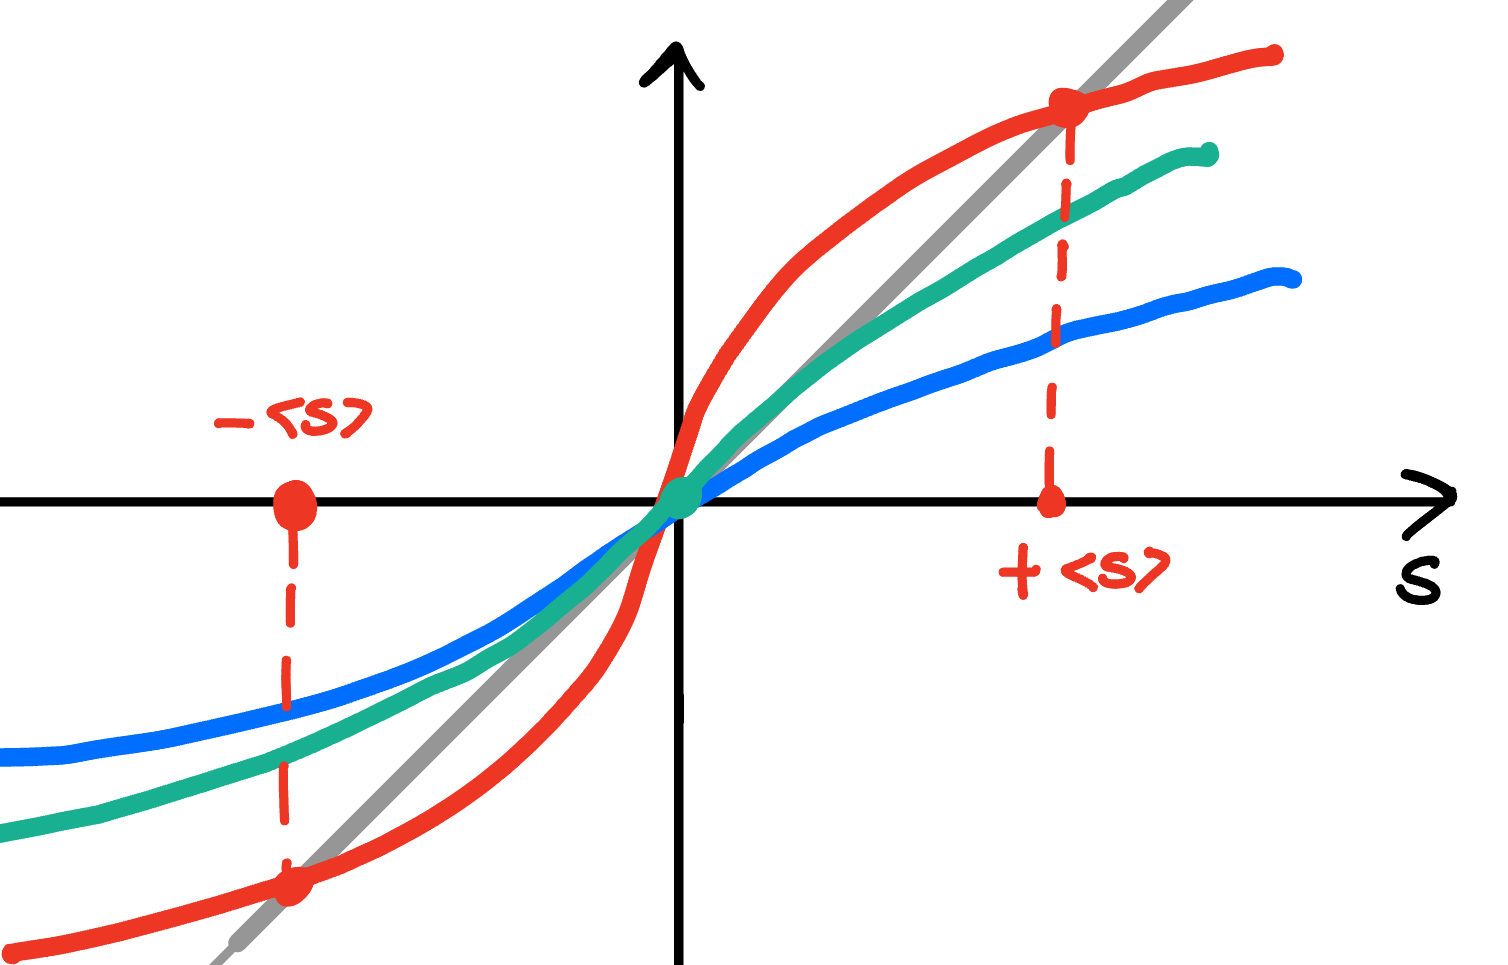
\includegraphics[width = 0.4\textwidth]{latex_source/images/ising/IMG_56FE6CFC861B-1.jpeg}
    \caption{\small Grey line is $y=s$, coloured lines are $y = \text{tanh}(\beta \left\langle k\right\rangle s)$, respectively for $\beta \left\langle k\right\rangle  > 1$ (red, ferromagnetic state), $\beta \left\langle k\right\rangle > 1$ (green, critical point) and $\beta \left\langle k\right\rangle < 1$ (blue, paramagnetic state).}
\end{figure}
\subsection*{Preliminary Montecarlo simulation on a 2D lattice}
{\small
An infinite regular $2-$ dimensional spin lattice with Hamiltonian given by [Eq: \ref{eq:ising_Hamiltonian}] exibits a second order phase transition at the critical temperature 
\begin{equation}
T_C = \frac{2\,}{\,\log{1 + \sqrt{2}}} \simeq 2.26
    \label{eq:onsager}
  \end{equation}  
For my simulation, I considered a lattice of $N = 20 \cdot 20 = 400$ nodes. I first simulated the dynamics at fixed temperature, to get an estimate of the number of steps required for the system to equilibrate. I found that $\simeq 200$ steps where sufficent for a lattice of this size [Fig \ref{fig:2d_relaxation}]. Then I simulated Ising over a broad range of temperatures around the expected critical temperature and computed the energy, magnetization, heat capacity and magnetic susceptibility [Fig: \ref{fig:2d_scaling}].
}
\begin{figure}[H]
    \centering
    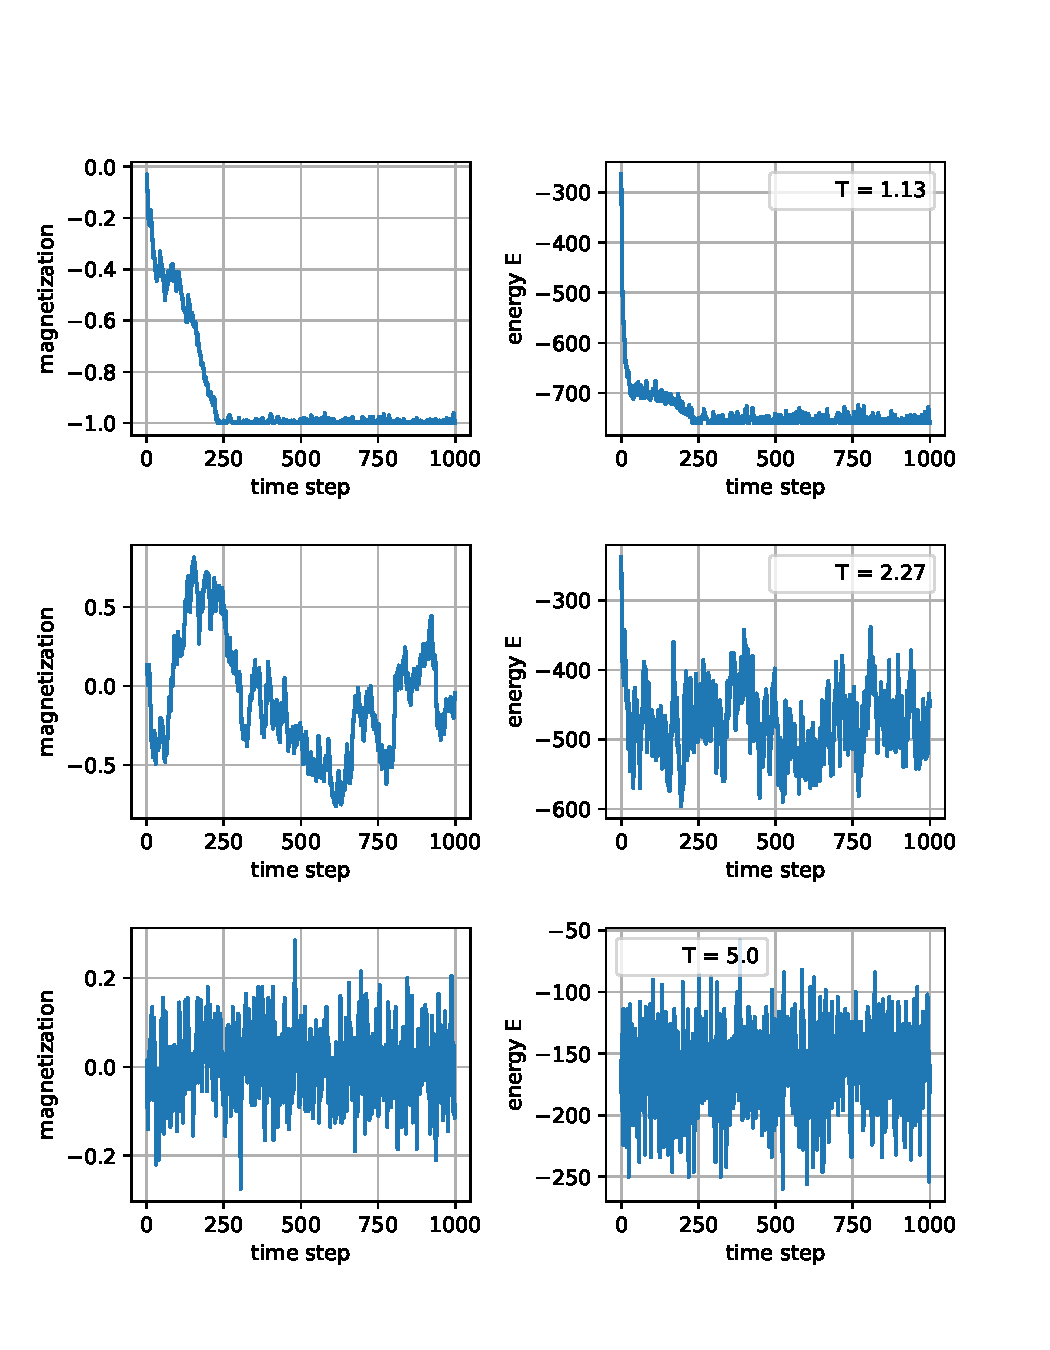
\includegraphics[width=0.8\linewidth]{latex_source/images/ising/2d_relaxation.pdf}
    \caption{{\small Time evolution of the magnetization and energy, respectively below, at and above the critical temperature [Eq:\,\ref{eq:onsager}].}}
    \label{fig:2d_relaxation}
\end{figure}

\begin{figure}[H]
    \centering
    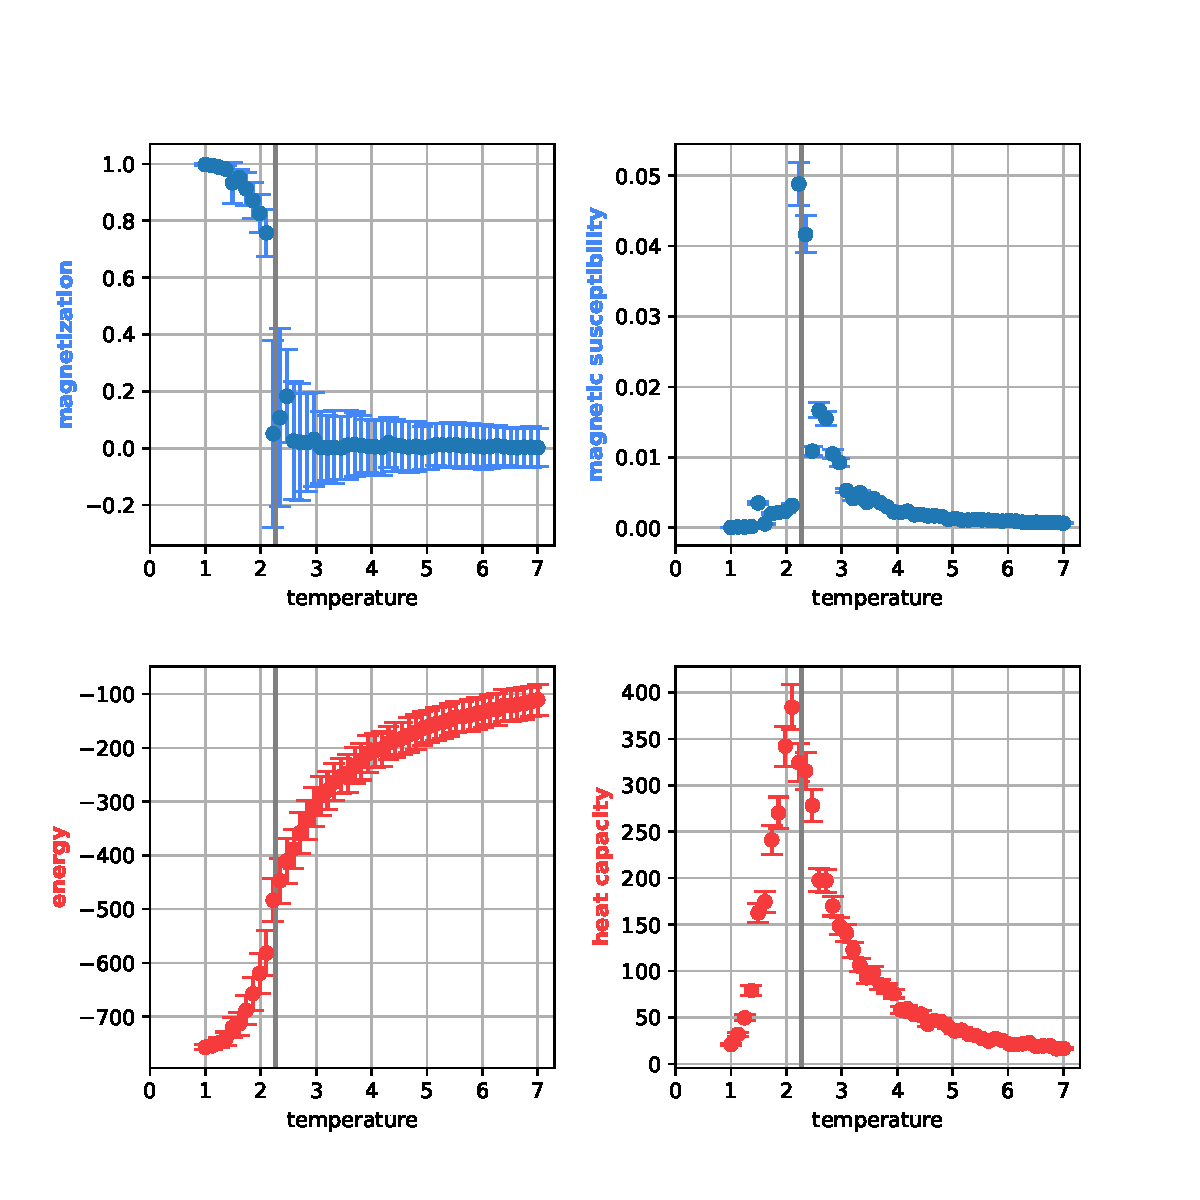
\includegraphics[width=\linewidth]{latex_source/images/ising/2d_scaling.pdf}
    \caption{Dependence of thermodynamic quantities on temperature, for a $2d$ regular square lattice of $400$ nodes. The vertical grey line marks the theoretical critical temperature [Eq: \ref{eq:onsager}]. One can see that the peaks of $C$ and $\chi$ are very close to the theoretical temperature. With $500$ equilibration steps and $500$ sweep steps at each temperature, the code took $12$ minutes to execute.}
    \label{fig:2d_scaling}
\end{figure}
}